\section{Stetige Verteilungen}

\subsection{Gleichverteilung}
Alle Ereignisse zwischen $a$ und $b$ sind gleich wahrscheinlich.

\vspace{10pt}

Notation:
\[
X \sim U(a,b)
\]

Dichtefunktion:
\[
f(x)=
\begin{cases}
	\frac{1}{b-a} & \text{für $a \leq x \leq b$} \\
	0 & \text{sonst} \\
\end{cases} 
\]

Verteilungsfunktion:
\[
F(x)=P[X \leq x]=
\begin{cases}
	0 & \text{für $x < a$} \\	
	\frac{x-a}{b-a} & \text{für $a \leq x \leq b$} \\
	1 & \text{für $x > b$} \\
\end{cases} 
\]

Erwartungswert:
\[
E[X]=\frac{b+a}{2}
\]

Varianz:
\[
Var[X]=\frac{(b-a)^2}{12}
\]

\subsection{Exponentialverteilung}
Die Exponentialverteilung ist ein Modell für Wartezeiten und Lebensdauern. Beispielanwendungen sind die Berechnung der Lebensdauer von Bauteilen und Zugverspätungen.

\vspace{10pt}

Notation:
\[
X \sim Exp(\lambda)
\]

Dichtefunktion:
\[
f(x)=
\begin{cases}
	\lambda e^{- \lambda x} & \text{für $x \geq 0$} \\
	0 & \text{für $x < 0$} \\
\end{cases} 
\]

Verteilungsfunktion:
\[
F(x)=P[X \leq x]=
\begin{cases}
	1-e^{- \lambda x} & \text{für $x \geq 0$} \\	
	0 & \text{für $x < 0$} \\
\end{cases} 
\]

Erwartungswert:
\[
E[X]=\frac{1}{\lambda}
\]

Varianz:
\[
Var[X]=\frac{1}{\lambda^{2}}
\]

\textbf{Bemerkungen:}
\begin{itemize}
\item Sind $X_1\sim Exp(\lambda_1), ..., X_n\sim Exp(\lambda_n)$ \emph{stochastisch unabhängig}, so ist $\min(X_1, ...,X_n)\sim Exp(\lambda_1+...+\lambda_n)$.
\item Die Summe von $n$ exponentialverteilten Zufallsvariablen mit \emph{gleichem Parameter} $\lambda$ ist gammaverteilt mit $\Gamma(n,\lambda)$.
\item Erwartungswert und Standardabweichung sind gleich ($E[X]=sd[X]$).
\end{itemize}

\textbf{Beispiel (Lebensdauer:)} Die Exponentialverteilung ist eine typische Lebensdauerverteilung. So ist z.B. die Lebensdauer von elektronischen Bauteilen häufig annähernd exponentialverteilt.

\subsection{Normalverteilung}
Die besondere Bedeutung der Normalverteilung beruht unter anderem auf dem zentralen Grenzwertsatz, der besagt, dass eine Summe von $n$ unabhängigen, identisch verteilten Zufallsvariablen mit endlicher Varianz im Grenzwert $n\rightarrow\infty$ normalverteilt ist.

\vspace{10pt}

Notation:
\[
X \sim N(\mu, \sigma^2)
\]

Dichtefunktion:
\[
f(x)=\frac{1}{\sigma \sqrt{2 \pi}}\cdot e^{-\frac{1}{2}\left(\frac{x-\mu}{\sigma}\right)^2}
\]

Verteilungsfunktion:
\[
F(x)=P[X \leq x]=\frac{1}{\sigma \sqrt{2 \pi}}\cdot\int\limits_{-\infty}^x e^{-\frac{1}{2}\left(\frac{t-\mu}{\sigma} \right)^2}dt
\]

Erwartungswert:
\[
E[X]=\mu
\]

Varianz:
\[
Var[X]=\sigma^2
\]

Transformation einer normalverteilten Zufallsvariable $X$ in eine standardnormalverteilte Zufallsvariable $Z$:
\[
Z=\frac{X-\mu}{\sigma}
\]

\textbf{Beispiel:} Gewicht von Kürbissen, Streuung von Messungen um den Mittelwert, Gewichte oder Grössen von Individuen in einer großen Bevölkerung.

\subsection{Standardnormalverteilung}
Notation:
\[
X \sim N(0,1)
\]

Dichtefunktion:
\[
\phi(u)=\frac{1}{\sqrt{2\pi}}\cdot e^{-\frac{u^2}{2}}
\]

Verteilungsfunktion:
\[
\Phi(u)=P[X \leq u]=\frac{1}{\sqrt{2\pi}}\cdot\int \limits_{-\infty}^u e^{-\frac{t^2}{2}}dt
\]

Erwartungswert:
\[
E[X]=0
\]

Varianz:
\[
Var[X]=1
\]

\textbf{Bemerkungen:}
\begin{itemize}
\item Die Standardnormalverteilung entspricht einer Normalverteilung mit den Parametern $\mu = 0$ und $\sigma = 1$.
\end{itemize}

\subsubsection{Tabelle ablesen}
$\Phi(x)$ bedeutet, dass man zu einem Wert $x$ die Wahrscheinlichkeit in der Tabelle auslesen will. $\Phi^{-1}(x)$ bedeutet, dass für eine Wahrscheinlichkeit der Tabellenwert ermittelt werden soll.

\begin{center}
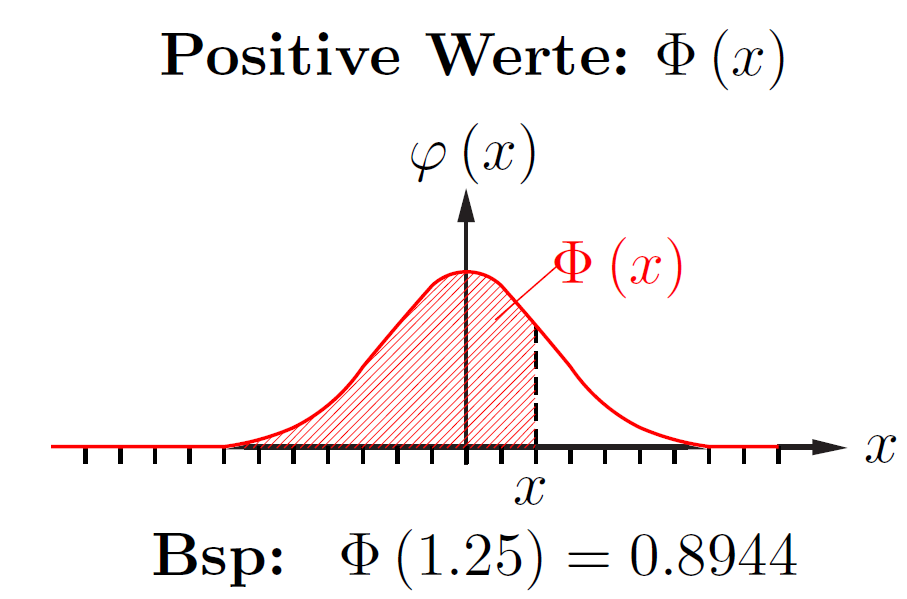
\includegraphics[width=45mm]{includes/standardnormalverteilung_tabelle1.png}
\end{center}
\begin{center}
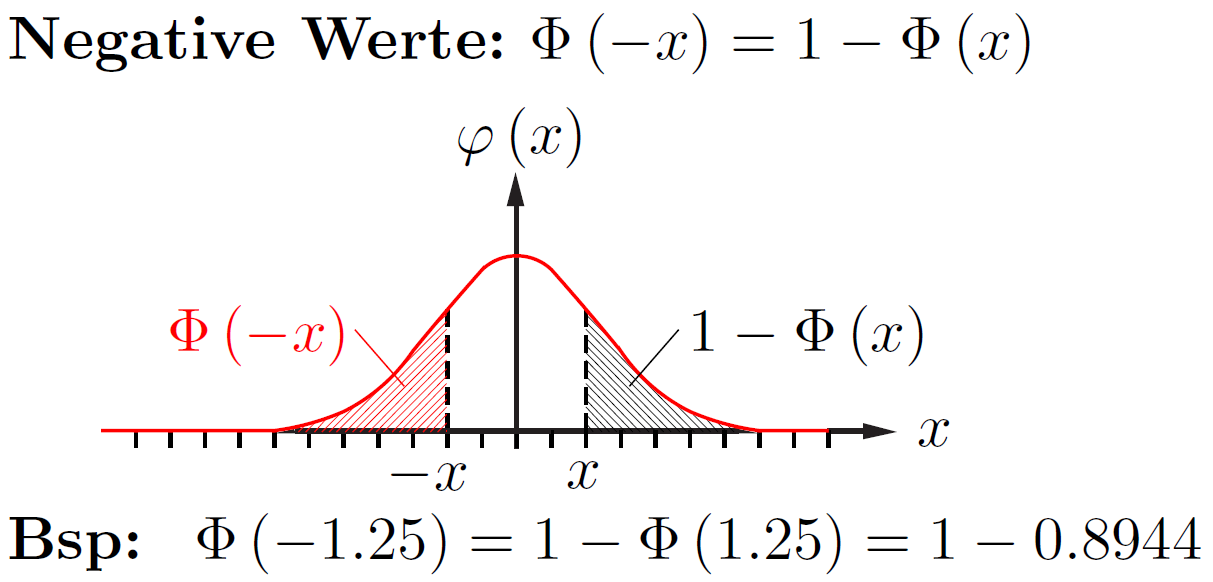
\includegraphics[width=60mm]{includes/standardnormalverteilung_tabelle2.png}
\end{center}

Für nicht tabellierte Werte:
\[
\Phi^{-1}(0.03)=-\Phi^{-1}(0.97)=-1.88
\]

Regeln zum Auslesen der Werte:
\begin{itemize}
\item Ist ein gesuchter Wert $c$ nicht tabelliert, so wird derjenige Wert $a$ oder $b$ genommen, der näher bei $c$ liegt.
\item Sind zwei Werte $a$ und $b$ gleich weit vom gesuchten Wert $c$ entfernt, so wird der Mittelwert von $a$ und $b$ verwendet.
\end{itemize}

\subsection{Pareto-Verteilung}
Die Pareto-Verteilung, ist eine stetige Wahrscheinlichkeitsverteilung auf einem rechtsseitigen unendlichen Intervall $[x_0, \infty)$. Eine stetige Zufallsvariable $X$ heisst pareto-verteilt $Par(\alpha, x_0)$ mit den Parametern $\alpha > 0$ und $x_0 > 0$, mit folgenden Eigenschaften:

\vspace{10pt}

Notation:
\[
X \sim Par(\alpha, x_0)
\]

Dichtefunktion:
\[
f(x) =\begin{cases}
			\dfrac{\alpha}{x_0}\left(\dfrac{x_0}{x}\right)^{\alpha + 1} & x \geq x_0\\
			0 & x < x_0
		\end{cases}
\]

Verteilungsfunktion:
\[
F(x; x_0, \alpha) = \begin{cases}
			1 - \left(\dfrac{x}{x_0}\right)^{-\alpha} & x \geq x_0, \alpha > 0,\\
			0 & \text{sonst}
		\end{cases}
\]

Erwartungswert:
\[
E[X] = \begin{cases}
			x_0\dfrac{\alpha}{\alpha - 1} & \alpha > 1\\
			\infty & \alpha \leq 1
		\end{cases}
\]

Varianz:
\[
Var[X] = \begin{cases}
			x_0^2 \left(\dfrac{\alpha}{\alpha - 2} - \dfrac{\alpha^2}{(\alpha - 1)^2}\right)\\
			= x_0^2 \dfrac{\alpha}{(\alpha - 2)(\alpha - 1)^2} & \alpha > 2\\
			\infty & \alpha \leq 2
		\end{cases}
\]

Standardabweichung:
\[
sd[X]=\dfrac{x_0}{\alpha - 1}\sqrt{\dfrac{\alpha}{\alpha - 2}} \text{ für } \alpha > 2
\]

\textbf{Beispiel:} Die Verteilung wurde zunächst zur Beschreibung der Einkommensverteilung Italiens verwendet. Paretoverteilungen finden sich charakteristischerweise dann, wenn sich zufällige, positive Werte über mehrere Größenordnungen erstrecken und durch das Einwirken vieler unabhängiger Faktoren zustande kommen.
